\chapter{जीव: अपने पर्यावरण से अंतःक्रिया करता एक तंत्र}\label{ch:b1:organism-environment}

जनवरी की एक सुबह कोई खरगोश किसी घास के मैदान के किनारे बैठा है। अगले
घंटे में वह सौ ग्राम घास खाएगा, कोई \qty{400}{L} हवा साँस में लेगा,
\qty{2}{\celsius} की हवा में अपने रोमों से ऊष्मा खोएगा, किसी गड्ढे से
पानी पिएगा, और किसी बाज़ की परछाईं मैदान पर पड़ते ही भाग खड़ा होगा।
इनमें से कुछ भी उसकी सीमा के आरपार किसी वस्तु के गुज़रे बिना संभव नहीं
है: पदार्थ भीतर और बाहर, ऊर्जा भीतर और बाहर, सूचना भीतर। दो सौ मीटर दूर
एक बाँज का पेड़ बिना हिले वही सब करता है --- कार्बन डाइऑक्साइड और प्रकाश
लेता है, अपने शिखर से बड़े जड़-तंत्र से पानी खींचता है, और वही पानी उसी
ठंडी हवा को दे देता है। यह अध्याय बताता है कि तंत्र के रूप में कोई \omterm{def:b1:organism-environment:organism}{जीव} है
क्या, उसका आकार यह क्यों तय करता है कि वह किस तरह बना है, बाहर सब कुछ
बदलते रहने पर भी वह अपने भीतर को स्थिर कैसे रखता है, और उसकी ऊर्जा-माँग
उसके द्रव्यमान के साथ किस तरह बढ़ती है। इस आरंभ के दो \omterm{def:b1:organism-environment:organism}{जीव}, एक स्तनधारी
और एक पुष्पी पौधा, पूरे वर्ष के आदर्श उदाहरण हैं।

\begin{omfigure}
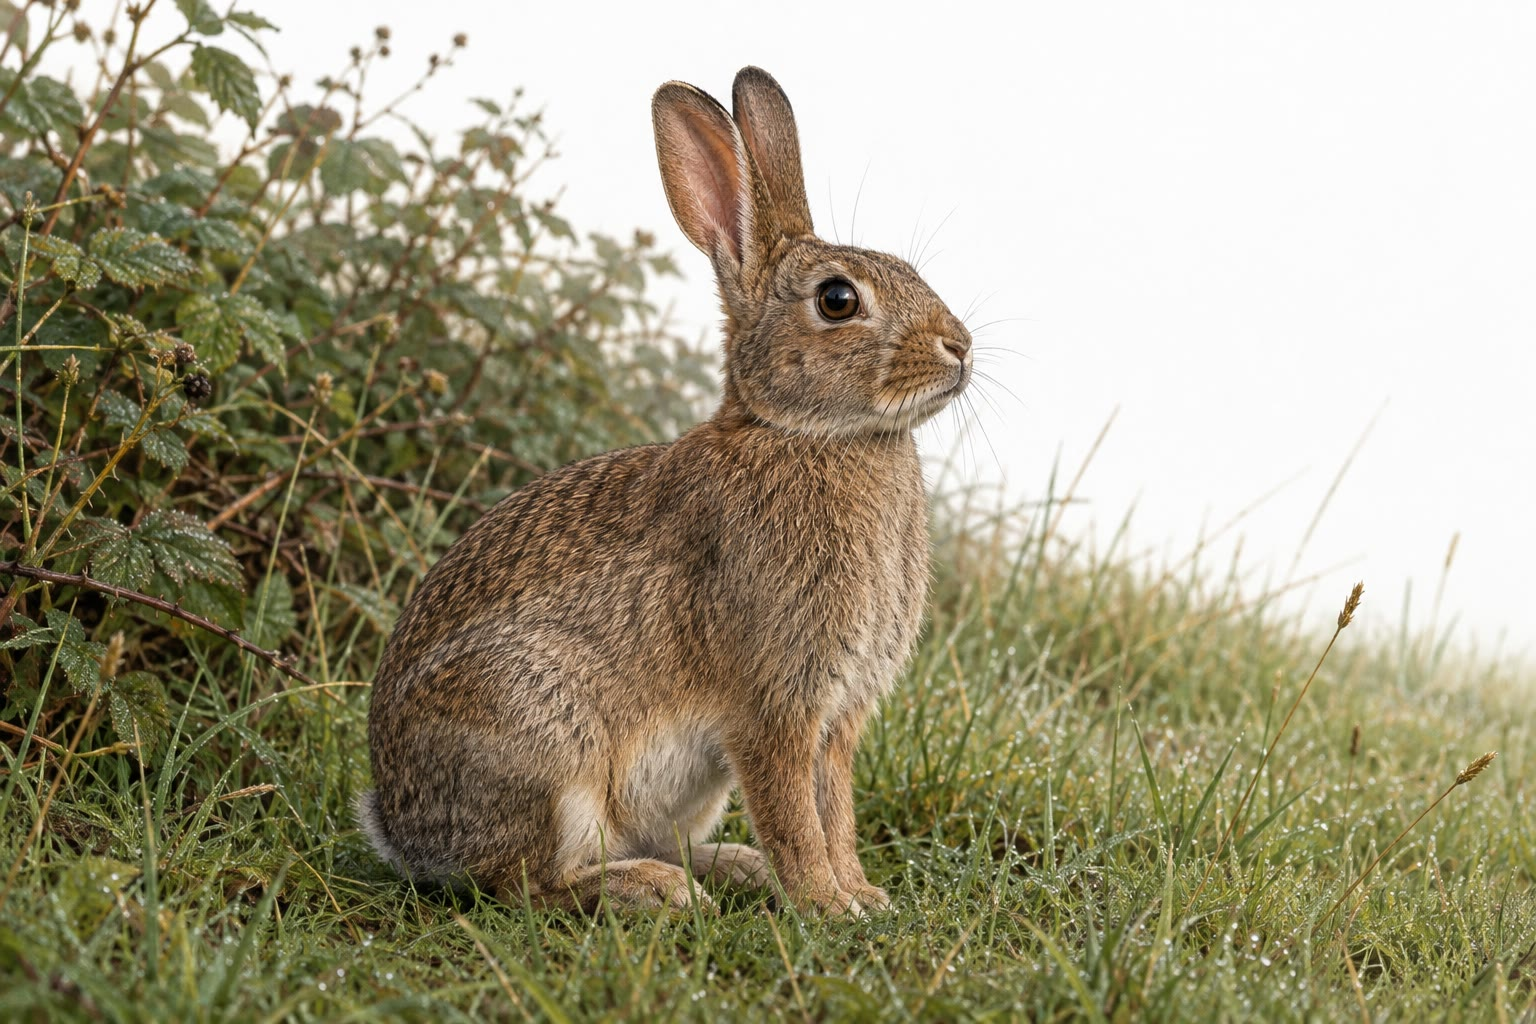
\includegraphics[width=0.62\linewidth]{images/book3/ai/b3-01-rabbit-field.jpg}

{\small घास के मैदान के किनारे एक जंगली खरगोश: एक घंटे में वह खाएगा,
साँस लेगा, ऊष्मा खोएगा, पानी पिएगा और भागेगा --- और इनमें से हर एक उसकी
सीमा के आरपार होता विनिमय है।}
\end{omfigure}

\section{एक विवृत तंत्र}

\begin{definition}[जीव, विवृत तंत्र]\label{def:b1:organism-environment:organism}
\emph{जीव}\index{जीव} कोई सजीव व्यष्टि है: एक परिबद्ध, स्वयं को बनाए
रखने वाला और स्वयं का जनन करने वाला तंत्र, जो एक कोशिका का बना है या फिर
अनेक ऐसी कोशिकाओं का जिनका उद्गम साझा है और कार्य भी साझा। वह एक
\emph{विवृत तंत्र}\index{विवृत तंत्र} है: पदार्थ और ऊर्जा उसकी सीमा के
आरपार निरंतर आते-जाते हैं, और जब तक वे आते-जाते हैं तभी तक वह जीवित
रहता है। किसी जीव का \emph{पर्यावरण}\index{पर्यावरण} उस सीमा के बाहर का
वह सब कुछ है जो उससे विनिमय करता है --- भौतिक माध्यम (हवा, जल, मिट्टी,
प्रकाश, ताप) और दूसरे जीव।
\end{definition}

\begin{proposition}[तीन विनिमय]\label{prop:b1:organism-environment:exchanges}
हर \omterm{def:b1:organism-environment:organism}{जीव} अपने पर्यावरण से तीन चीज़ों का विनिमय करता है:
\begin{itemize}
  \item \emph{पदार्थ}\index{पदार्थ विनिमय}: वह पोषक तत्व, जल और गैसें
        भीतर लेता है और अपशिष्ट, गैसें और जल छोड़ता है;
  \item \emph{ऊर्जा}\index{ऊर्जा विनिमय}: वह ऊर्जा या तो प्रकाश के रूप
        में लेता है (\omterm{def:b1:organism-environment:trophy}{स्वपोषी}) या भोजन की रासायनिक ऊर्जा के रूप
        (\omterm{def:b1:organism-environment:trophy}{परपोषी}), और उसे लगभग पूरा ऊष्मा के रूप में छोड़ता है;
  \item \emph{सूचना}\index{सूचना विनिमय}: वह पर्यावरण के संकेतों
        (प्रकाश, रसायन, ताप, स्पर्श, ध्वनि) को भाँपता है और उन पर
        अनुक्रिया करता है।
\end{itemize}
जिस अवधि में \omterm{def:b1:organism-environment:organism}{जीव} न बढ़ता है न घटता, उस अवधि में उसका बहीखाता बंद रहता है:
भीतर आया पदार्थ बाहर गए पदार्थ के बराबर है, और भीतर आई ऊर्जा बाहर गई
ऊष्मा और बाहर पर किए गए कार्य के योग के बराबर।
\end{proposition}
\begin{proof}
पहले दो द्रव्यमान और ऊर्जा के संरक्षण से निकलते हैं, जिन्हें सीमा के भीतर
के आयतन पर लगाया जाता है: जो कुछ संचित होता है वह भीतर आने और बाहर जाने
का अंतर है, और स्थायी अवस्था का \omterm{def:b1:organism-environment:organism}{जीव} कुछ भी संचित नहीं करता। जो रासायनिक
ऊर्जा नए जैवभार के रूप में संचित नहीं होती वह अंत में ऊष्मा बनती है,
क्योंकि \omterm{def:b1:organism-environment:organism}{जीव} की हर अभिक्रिया अपनी मुक्त ऊर्जा ऊष्मा के रूप में क्षय करती
है, और बाहर पर किया गया यांत्रिक कार्य (चलना, उठाना) ही एकमात्र दूसरा
निकास है। तीसरा यह प्रेक्षण है कि कोई भी \omterm{def:b1:organism-environment:organism}{जीव} अपने परिवेश के प्रति जड़
नहीं है।
\end{proof}

\begin{omfigure}
\begin{tikzpicture}[font=\footnotesize, >=Stealth, line cap=round]
  \draw[very thick, omDef, fill=omDef!6, rounded corners=12pt] (0,0) rectangle (4.4,3.4);
  \node[font=\small\bfseries, omDef] at (2.2,2.95) {जीव};
  \node[align=center] at (2.2,1.5) {आंतरिक पर्यावरण\\ कोशिकाएँ, ऊतक, अंग\\ रासायनिक कार्य, वृद्धि,\\ गति, जनन};
  % matter in / out
  \draw[->, thick, omProp] (-1.3,2.6) -- (0,2.6) node[pos=0, left, align=right] {पोषक तत्व, जल,\\ $\mathrm{O_2}$ या $\mathrm{CO_2}$};
  \draw[->, thick, omProp] (4.4,2.6) -- (5.7,2.6) node[right, align=left] {अपशिष्ट, जल,\\ $\mathrm{CO_2}$ या $\mathrm{O_2}$};
  % energy
  \draw[->, thick, omThm] (-1.3,1.5) -- (0,1.5) node[pos=0, left, align=right] {ऊर्जा: प्रकाश, या\\ भोजन की रासायनिक ऊर्जा};
  \draw[->, thick, omThm] (4.4,1.5) -- (5.7,1.5) node[right, align=left] {ऊष्मा, और बाहर पर\\ किया गया कार्य};
  % information
  \draw[->, thick, omExo] (-1.3,0.5) -- (0,0.5) node[pos=0, left, align=right] {सूचना: प्रकाश,\\ रसायन, ताप};
  \draw[->, thick, omExo] (4.4,0.5) -- (5.7,0.5) node[right, align=left] {अनुक्रियाएँ: गति,\\ स्राव, वृद्धि};
\end{tikzpicture}

{\small \omterm{def:b1:organism-environment:organism}{विवृत तंत्र} के रूप में \omterm{def:b1:organism-environment:organism}{जीव}: पदार्थ (नारंगी), ऊर्जा (लाल) और
सूचना (हरा) उसकी सीमा के आरपार जाते हैं। स्थायी अवस्था का \omterm{def:b1:organism-environment:organism}{जीव} उतना ही
पदार्थ छोड़ता है जितना लेता है, और अपनी लगभग सारी ली हुई ऊर्जा को ऊष्मा
में बदल देता है।}
\end{omfigure}

\begin{definition}[स्वपोषी, परपोषी]\label{def:b1:organism-environment:trophy}
कोई \omterm{def:b1:organism-environment:organism}{जीव} तब \emph{स्वपोषी}\index{स्वपोषण} होता है जब वह अपना कार्बनिक
पदार्थ खनिज कार्बन (कार्बन डाइऑक्साइड) से, किसी बाहरी ऊर्जा-स्रोत की
सहायता से बनाता है --- \emph{प्रकाशस्वपोषियों}\index{प्रकाशस्वपोषी}
(पौधे, शैवाल, सायनोबैक्टीरिया) के लिए वह स्रोत प्रकाश है, और
\emph{रसायनस्वपोषियों}\index{रसायनस्वपोषी} के लिए खनिज यौगिकों का
ऑक्सीकरण। वह तब \emph{परपोषी}\index{परपोषण} होता है जब उसे दूसरे \omterm{def:b1:organism-environment:organism}{जीवों}
का बनाया कार्बनिक पदार्थ भीतर लेना पड़ता है, जो उसे उसका कार्बन और उसकी
ऊर्जा दोनों देता है (जंतु, कवक, अधिकांश जीवाणु)।
\end{definition}

\begin{example}[खरगोश और बाँज]\label{ex:b1:organism-environment:rabbitoak}
खरगोश की सौ ग्राम घास पचने के बाद लगभग \qty{500}{kJ} रासायनिक ऊर्जा
देती है और उस हर अणु का कार्बन भी जो वह बनाएगा; जो ऑक्सीजन वह साँस में
लेता है वह उसे उस भोजन का ऑक्सीकरण करने देती है, और जो कार्बन
डाइऑक्साइड वह छोड़ता है वह वही कार्बन है जो बाहर जा रहा है। बाँज का
लेन-देन उल्टा है: कार्बन डाइऑक्साइड भीतर, ऑक्सीजन बाहर, और ऊर्जा प्रकाश
के रूप में --- दोपहर में उसके शिखर पर पड़ते कोई \qty{5}{kW}, जिनका एक
प्रतिशत से भी कम वह शर्करा के रूप में संचित करता है। दोनों अपनी संसाधित
ऊर्जा का लगभग सारा भाग ऊष्मा के रूप में छोड़ते हैं: खरगोश के रोम गरम हैं,
और बाँज की पत्तियाँ उसी वाष्पन से ठंडी होती हैं जिसे उसका अपना
प्रकाश-अवशोषण चलाता है।
\end{example}

\section{संगठन के पैमाने और आकार की समस्या}

\begin{definition}[संगठन के स्तर]\label{def:b1:organism-environment:levels}
सजीव पदार्थ अंतर्निहित \emph{संगठन के स्तरों}\index{संगठन के स्तर} में
सजा है, जिनमें हर स्तर अपने नीचे वाले की इकाइयों से बना है और हर स्तर के
वे गुण हैं जो नीचे वाले के नहीं: अणु ($\qty{1}{nm}$), कोशिकाएँ
($\qtyrange{1}{100}{\micro m}$), ऊतक, अंग ($\qtyrange{1}{100}{mm}$), अंग
तंत्र, \omterm{def:b1:organism-environment:organism}{जीव} ($\qty{1}{\micro m}$ से $\qty{100}{m}$ तक), और उसके ऊपर
आबादी, समुदाय, पारितंत्र और जैवमंडल। कोशिका श्वसन करती है; अणु नहीं।
आबादी विकसित होती है; \omterm{def:b1:organism-environment:organism}{जीव} नहीं।
\end{definition}

\begin{proposition}[सतह और आयतन]\label{prop:b1:organism-environment:sv}
एक ही आकृति और अभिलक्षणिक माप $L$ के पिंडों के लिए सतह $L^2$ की तरह
बढ़ती है और आयतन $L^3$ की तरह, इसलिए सतह-आयतन अनुपात $1/L$ की तरह
घटता है:
\[
\frac{S}{V} \propto \frac{1}{L}, \qquad
\frac{S}{V}\Big|_{\text{गोला}} = \frac{4\pi r^2}{\tfrac{4}{3}\pi r^3} = \frac{3}{r}.
\]
जो कुछ \omterm{def:b1:organism-environment:organism}{जीव} विनिमय करता है वह किसी सतह से होकर जाता है, और जो कुछ वह
खपाता है वह उसके आयतन के समानुपाती है: कोई बड़ा \omterm{def:b1:organism-environment:organism}{जीव} अपने आयतन को अपनी
बाहरी सतह से नहीं खिला सकता।
\end{proposition}
\begin{proof}
किसी आकृति को $k$ गुणक से बड़ा करने पर हर क्षेत्रफल $k^2$ से और हर आयतन
$k^3$ से गुणा हो जाता है; अनुपात $1/k$ से गुणा होता है। गोले के लिए यह
सूत्र यथार्थ है।
\end{proof}

\begin{example}[एक जीवाणु और एक मनुष्य]\label{ex:b1:organism-environment:svnumbers}
$\qty{0.5}{\micro m}$ त्रिज्या के किसी जीवाणु के लिए
$S/V = 3/r = \qty{6e6}{m^{-1}}$: उसके कोशिकाद्रव्य का हर घन माइक्रोमीटर
बाहर से आधे माइक्रोमीटर के भीतर है, और उसकी झिल्ली से होता विसरण ही उसे
पूरा खिला देता है। \qty{70}{L} के गोले के रूप में लिए गए मनुष्य के लिए
$r = \qty{0.26}{m}$ और $S/V = \qty{12}{m^{-1}}$, यानी पाँच लाख गुना कम।
त्वचा, लगभग \qty{2}{m^2}, उतनी ऑक्सीजन नहीं दे सकती जितनी \qty{70}{kg}
ऊतक खपाता है; वक्ष के भीतर मुड़ा हुआ फेफड़ा \qty{100}{m^2} देता है, और
तीन बार मुड़ी हुई आँत \qty{30}{m^2}।
\end{example}

\begin{omfigure}
\begin{tikzpicture}
\begin{axis}[
  xbar, bar width=8pt,
  width=0.82\linewidth, height=6.2cm,
  axis x line=bottom, axis y line=left,
  xmode=log, log origin=infty, xmin=0.5, xmax=3000,
  xlabel={विनिमय सतह (\unit{m^2})},
  xlabel style={font=\small, at={(axis description cs:0.5,-0.13)}, anchor=north},
  symbolic y coords={human skin, human lung, human small intestine, oak leaves, rye root system, rye root hairs},
  yticklabels={मनुष्य की त्वचा, मनुष्य का फेफड़ा, मनुष्य की छोटी आँत, बाँज की पत्तियाँ, राई का जड़-तंत्र, राई के मूलरोम},
  ytick=data, tick label style={font=\small},
  enlarge y limits=0.12,
  nodes near coords, nodes near coords style={font=\scriptsize, anchor=west},
  point meta=rawx,
]
\addplot[fill=omDef!45, draw=omDef] coordinates
  {(2,human skin) (100,human lung) (30,human small intestine) (300,oak leaves) (240,rye root system) (400,rye root hairs)};
\end{axis}
\end{tikzpicture}

{\small \omterm{prop:b1:organism-environment:surfaces}{विनिमय सतहें}, लघुगणकीय पैमाने पर। मनुष्य की बाहरी सतह
\qty{2}{m^2} है; उसके भीतर मुड़ी हुई सतहें, और जो सतहें पौधा हवा और
मिट्टी में फैलाता है, उनसे दस से दो सौ गुना बड़ी हैं। (एक ही राई का पौधा
चार महीने डिब्बे में उगाया गया: \qty{240}{m^2} जड़ें और \qty{400}{m^2}
मूलरोम।)}
\end{omfigure}

\begin{proposition}[विनिमय सतहें मुड़ी हुई, पतली और संवातित होती हैं]\label{prop:b1:organism-environment:surfaces}
लगभग एक मिलीमीटर से बड़े आकार पर कोई \omterm{def:b1:organism-environment:organism}{जीव} अपनी बाहरी सतह से होते विसरण से
नहीं खाया-पिलाया जा सकता। इसलिए किसी भी आकार के बहुकोशिकीय \omterm{def:b1:organism-environment:organism}{जीव}
\emph{विशिष्ट विनिमय सतहें}\index{विनिमय सतह} रखते हैं, जिनकी साझा
अभिकल्पना एक ही समस्या को चार तरह से हल करती है: बड़ा क्षेत्रफल (मुड़ाव:
रसांकुर, कूपिकाएँ, क्लोम-पटलिकाएँ, मूलरोम, पर्ण-फलक), छोटी मोटाई (दोनों
माध्यमों के बीच एक कोशिका-परत या उससे भी कम), बाहर की ओर नवीकृत होता
माध्यम (संवातन, जल-धारा, वाष्पोत्सर्जन-धारा), और भीतर की ओर कोई
अभिगमन-तंत्र (रक्त, रस) जो सतह पार करने वाली वस्तु को शेष आयतन तक
पहुँचाता है।
\end{proposition}
\begin{proof}
फ़िक का नियम (\cref{ch:b1:membranes-transport}) किसी सतह के आरपार फ्लक्स
को क्षेत्रफल के, सांद्रता-अंतर के और मोटाई के व्युत्क्रम के समानुपाती
देता है; बाहरी माध्यम का नवीकरण सांद्रता-अंतर को बड़ा बनाए रखता है; और
अभिगमन-तंत्र जो पार कर चुका है उसे हटाकर भीतरी सांद्रता कम रखता है। इन
चारों में से हर एक फ्लक्स बढ़ाता है; बड़े \omterm{def:b1:organism-environment:organism}{जीव} को चारों चाहिए।
\end{proof}

\section{आंतरिक पर्यावरण और समस्थापन}

\begin{definition}[आंतरिक पर्यावरण]\label{def:b1:organism-environment:milieu}
किसी बहुकोशिकीय जंतु में अधिकांश कोशिकाएँ बाहरी संसार के संपर्क में नहीं
होतीं, बल्कि किसी \emph{आंतरिक पर्यावरण}\index{आंतरिक पर्यावरण} में डूबी
रहती हैं: वह बाह्यकोशिकीय द्रव (रक्त प्लाज़्मा, लसीका, कोशिकाओं के बीच
का अंतराली द्रव) जिसका संघटन, ताप और आयतन \omterm{def:b1:organism-environment:organism}{जीव} नियंत्रित करता है।
कोशिकाएँ इसी द्रव से विनिमय करती हैं; और यह द्रव विशिष्ट सतहों से होकर
बाहर से विनिमय करता है। यह विचार क्लोद बर्नार का है (1865): आंतरिक
पर्यावरण की अचरता ही स्वतंत्र और स्वाधीन जीवन की शर्त है।
\end{definition}

\begin{definition}[समस्थापन]\label{def:b1:organism-environment:homeostasis}
\emph{समस्थापन}\index{समस्थापन} \omterm{def:b1:organism-environment:milieu}{आंतरिक पर्यावरण} के किसी नियंत्रित चर
(ताप, ग्लूकोज़ सांद्रता, pH, परासरणीयता, रक्तदाब) को बाहरी परिवर्तनों के
बावजूद किसी \emph{नियत बिंदु}\index{नियत बिंदु} के पास बनाए रखना है। यह
\emph{ऋण प्रतिपुष्टि}\index{ऋण प्रतिपुष्टि} से सधता है: कोई
\emph{संवेदक} उस चर को मापता है, कोई समाकलक केंद्र उसकी तुलना नियत बिंदु
से करता है, और कोई \emph{प्रभावक} उस दिशा में काम करता है जो विचलन को
रद्द करती है। वह चर स्थिर नहीं रहता, बल्कि नियत बिंदु के आसपास एक सँकरी
पट्टी में दोलन करता है।
\end{definition}

\begin{omfigure}
\begin{tikzpicture}[font=\small, >=Stealth, line cap=round,
  box/.style={draw, thick, rounded corners=4pt, minimum height=9mm, minimum width=26mm, align=center, fill=white}]
  \node[box, fill=omDef!10] (var) at (0,0) {नियंत्रित चर\\ (जैसे शरीर का ताप)};
  \node[box, fill=omProp!10] (sens) at (4.6,1.5) {संवेदक\\ (तापग्राही)};
  \node[box, fill=omThm!10] (int) at (4.6,-1.5) {समाकलक केंद्र\\ (हाइपोथैलेमस)};
  \node[box, fill=omExo!10] (eff) at (0,-3.0) {प्रभावक\\ (कँपकँपी, वाहिकाएँ, पसीना)};
  \node[font=\footnotesize, align=center] (set) at (8.4,-1.5) {नियत बिंदु\\ $\qty{37}{\celsius}$};
  \draw[->, thick] (var.east) -- ++(1.0,0) |- (sens.west);
  \draw[->, thick] (sens.south) -- (int.north) node[midway, right, font=\footnotesize] {मापा गया मान};
  \draw[->, thick] (set.west) -- (int.east);
  \draw[->, thick] (int.south) -- ++(0,-0.6) -| (eff.east) ;
  \draw[->, thick] (eff.north) -- (var.south) node[midway, left, font=\footnotesize, align=right] {सुधार,\\ विचलन के विपरीत};
  \draw[->, thick, gray] (-3.6,0.9) -- (var.north west) node[pos=0, above, font=\footnotesize, gray, align=center] {विक्षोभ\\ (ठंडी हवा)};
\end{tikzpicture}

{\small एक ऋण-प्रतिपुष्टि पाश। संवेदक चर की सूचना देता है, केंद्र उसकी
तुलना \omterm{def:b1:organism-environment:homeostasis}{नियत बिंदु} से करता है, और प्रभावक चर को वापस धकेलते हैं। सुधार का
चिह्न सदा विचलन के चिह्न के विपरीत होता है --- इसीलिए \emph{ऋण}।}
\end{omfigure}

\begin{proposition}[अंतस्तापी और बाह्यतापी]\label{prop:b1:organism-environment:thermo}
किसी \emph{बाह्यतापी}\index{बाह्यतापी} \omterm{def:b1:organism-environment:organism}{जीव} (अधिकांश अकशेरुकी, मछलियाँ,
उभयचर, सरीसृप) के शरीर का ताप पर्यावरण के ताप के पीछे-पीछे चलता है; उसकी
\omterm{def:b1:organism-environment:allometry}{उपापचय दर} ताप के साथ बढ़ती है, हर \qty{10}{\celsius} पर मोटे तौर पर
दुगुनी। कोई \emph{अंतस्तापी}\index{अंतस्तापी} \omterm{def:b1:organism-environment:organism}{जीव} (स्तनधारी, पक्षी)
उपापचय से ऊष्मा बनाकर अपने शरीर का ताप किसी \omterm{def:b1:organism-environment:homeostasis}{नियत बिंदु} पर रखता है।
परिवेशी तापों के किसी \emph{तापउदासीन क्षेत्र}\index{तापउदासीन क्षेत्र}
में वह यह अपनी आधारी दर पर कर लेता है, और केवल कुचालकता तथा त्वचा में
रक्त-प्रवाह समायोजित करता है; उस क्षेत्र से नीचे हवा के ठंडा होते जाने पर
उसकी \omterm{def:b1:organism-environment:allometry}{उपापचय दर} रैखिक रूप से बढ़ती है, क्योंकि ऊष्मा-ह्रास ताप-अंतर के
समानुपाती है और उसकी भरपाई ऊष्मा-उत्पादन से करनी पड़ती है; और उससे ऊपर,
वाष्पन से ठंडा होने में जल और ऊर्जा दोनों ख़र्च होते हैं।
\end{proposition}
\begin{proof}[आंशिक उपपत्ति]
$T_b$ ताप के किसी पिंड के लिए, जो $T_a$ ताप की हवा में है, प्रति एकांक
समय उसकी सतह से खोई ऊष्मा $P = hS\,(T_b - T_a)$ है (न्यूटन का शीतलन नियम), जिसमें
$h$ वह गुणांक है जिसे रोम, पंख या वसा घटा देते हैं। ताप स्थिर रहने के
लिए ऊष्मा-उत्पादन $P$ के बराबर होना चाहिए, इसलिए \omterm{prop:b1:organism-environment:thermo}{तापउदासीन क्षेत्र} से
नीचे वह $T_a$ में रैखिक है, और उसकी प्रवणता $-hS$ है। उस क्षेत्र का
अस्तित्व और उसकी चौड़ाई, जहाँ $h$ स्वयं समायोजित होता है (रोम फुलाना,
त्वचा की वाहिकाएँ सिकोड़ना), शरीरक्रियात्मक तथ्य हैं, समीकरण के परिणाम
नहीं।
\end{proof}

\begin{omfigure}
\begin{tikzpicture}
\begin{axis}[
  width=0.9\linewidth, height=6.4cm,
  axis x line=bottom, axis y line=left,
  xmin=-10, xmax=45, ymin=0, ymax=5.2,
  xlabel={परिवेशी ताप (\unit{\celsius})}, ylabel={उपापचय दर (आधारी दर के गुणज)},
  xlabel style={font=\small, at={(axis description cs:0.5,-0.12)}, anchor=north},
  ylabel style={font=\small},
  tick label style={font=\small}, xtick={-10,0,10,20,30,40}, ytick={1,2,3,4,5},
  clip=false, legend style={font=\small, at={(0.97,0.97)}, anchor=north east, draw=none},
]
\addplot[very thick, omThm] coordinates {(-10,4.6) (0,3.4) (10,2.2) (20,1.0) (30,1.0) (33,1.05) (38,1.5) (42,2.2)};
\addlegendentry{अंतस्तापी (एक चूहा)}
\addplot[very thick, omDef] coordinates {(-10,0.05) (0,0.12) (10,0.25) (20,0.5) (30,1.0) (40,2.0)};
\addlegendentry{बाह्यतापी (एक छिपकली)}
\draw[dashed, gray] (axis cs:20,0) -- (axis cs:20,1.0);
\draw[dashed, gray] (axis cs:30,0) -- (axis cs:30,1.0);
\node[font=\scriptsize, anchor=south, align=center] at (axis cs:25,1.15) {तापउदासीन\\ क्षेत्र};
\node[font=\scriptsize, anchor=west, align=left] at (axis cs:11,3.5) {प्रवणता $= -hS$: ऊष्मा-उत्पादन\\ ऊष्मा-ह्रास की बराबरी करता है};
\end{axis}
\end{tikzpicture}

{\small परिवेशी ताप के सापेक्ष \omterm{def:b1:organism-environment:allometry}{उपापचय दर}। \omterm{prop:b1:organism-environment:thermo}{अंतस्तापी} की दर उसके \omterm{prop:b1:organism-environment:thermo}{तापउदासीन
क्षेत्र} में सबसे कम है और हवा के ठंडा होते जाने पर रैखिक रूप से बढ़ती है;
\omterm{prop:b1:organism-environment:thermo}{बाह्यतापी} की दर बस ताप के पीछे चलती है, हर दस डिग्री पर दुगुनी होती
हुई।}
\end{omfigure}

\begin{example}[दो डिग्री की एक रात]\label{ex:b1:organism-environment:night}
आरंभ वाला खरगोश, अपने बिल में विश्राम करते हुए, अपने \omterm{prop:b1:organism-environment:thermo}{तापउदासीन क्षेत्र}
में लगभग \qty{6}{W} ऊष्मा बनाता है। बाहर \qty{2}{\celsius} पर, जो उस
क्षेत्र के निचले किनारे से बीस डिग्री नीचे है, उसका उत्पादन बढ़कर लगभग
\qty{12}{W} होना चाहिए: कँपकँपी और उसके वसा-भंडार का ऑक्सीकरण यह अंतर
पूरा करते हैं, और उसका चरने का समय लंबा हो जाता है। उसी ढलान पर बैठी
छिपकली ठंड से नहीं लड़ती: उसका शरीर \qty{3}{\celsius} पर उतर आता है,
उसका उपापचय अपने ग्रीष्मकालीन मान का बीसवाँ भाग रह जाता है, और सूरज लौटने
तक वह हिलती नहीं।
\end{example}

\section{उपापचय दर और शरीर-द्रव्यमान}

\begin{definition}[उपापचय दर, अपमिति]\label{def:b1:organism-environment:allometry}
किसी \omterm{def:b1:organism-environment:organism}{जीव} की \emph{उपापचय दर}\index{उपापचय दर} $B$ वह दर है जिससे वह
रासायनिक ऊर्जा को रूपांतरित करता है; इसे वाट में, ऊष्मा-उत्पादन या
ऑक्सीजन-खपत के रूप में मापा जाता है ($\qty{1}{L}$ $\mathrm{O_2}$ की खपत
$\approx \qty{20}{kJ}$)। \emph{आधारी उपापचय दर}\index{आधारी उपापचय दर}
वह दर है जो अपने \omterm{prop:b1:organism-environment:thermo}{तापउदासीन क्षेत्र} में विश्राम कर रहे, भूखे \omterm{prop:b1:organism-environment:thermo}{अंतस्तापी} की
होती है। किसी राशि $Y$ के बारे में कहा जाता है कि वह शरीर-द्रव्यमान $M$
के साथ \emph{अपमितीय}\index{अपमिति} रूप से बदलती है जब
$Y = a\,M^{b}$ हो और घातांक $b \neq 1$ हो; लघुगणक--लघुगणक आलेख पर यह
संबंध $b$ प्रवणता की एक सरल रेखा है।
\end{definition}

\begin{theorem}[क्लाइबर का नियम]\label{thm:b1:organism-environment:kleiber}
\index{क्लाइबर का नियम}
छछूँदर से लेकर व्हेल तक, स्तनधारियों और पक्षियों में \omterm{def:b1:organism-environment:allometry}{आधारी उपापचय दर}
शरीर-द्रव्यमान की तीन-चौथाई घात की तरह बदलती है:
\[
B \approx \qty{3.4}{W}\times\left(\frac{M}{\qty{1}{kg}}\right)^{3/4}.
\]
इसलिए \emph{प्रति एकांक द्रव्यमान} दर $B/M$ $M^{-1/4}$ की तरह घटती है:
चूहे का हर ग्राम हाथी के हर ग्राम से लगभग बीस गुना तेज़ी से ऊर्जा जलाता
है।
\end{theorem}
\begin{proof}[साक्ष्य]
क्लाइबर (1932) ने \qty{20}{g} से \qty{600}{kg} तक के जंतुओं का मापा गया
ऊष्मा-उत्पादन उनके द्रव्यमान के सापेक्ष लघुगणकीय अक्षों पर आलेखित किया और
$0.74$ प्रवणता की एक सरल रेखा पाई, न कि $0.67$, जिसकी भविष्यवाणी
सतह-समानुपाती ऊष्मा-ह्रास करता। तब से यह रेखा द्रव्यमान की आठ कोटियों तक
बढ़ाई जा चुकी है और प्रवणता कुछ सौवें भाग के भीतर वही रही है। घातांक
$3/4$ क्यों है और $2/3$ क्यों नहीं, यह अब भी विवादित है: सबसे आगे चल रही
व्याख्या इसे उन शाखित जालों (वाहिकाएँ, वायुमार्ग) की ज्यामिति से जोड़ती
है जो हर कोशिका तक ऑक्सीजन पहुँचाते हैं।
\end{proof}

\begin{omfigure}
\begin{tikzpicture}
\begin{loglogaxis}[
  width=0.9\linewidth, height=6.6cm,
  axis x line=bottom, axis y line=left,
  xmin=0.005, xmax=20000, ymin=0.05, ymax=6000,
  xlabel={शरीर-द्रव्यमान (\unit{kg})}, ylabel={आधारी उपापचय दर (\unit{W})},
  xlabel style={font=\small, at={(axis description cs:0.5,-0.12)}, anchor=north},
  ylabel style={font=\small},
  tick label style={font=\small},
  xtick={0.01,0.1,1,10,100,1000,10000}, ytick={0.1,1,10,100,1000},
  log ticks with fixed point,
  clip=false,
]
\addplot[thick, omThm, domain=0.005:20000, samples=40] {3.4*x^0.75};
\addplot[only marks, mark=*, mark size=2pt, omDef] coordinates
  {(0.02,0.19) (0.3,1.3) (3,7.5) (70,80) (500,360) (4000,1700)};
\node[font=\scriptsize, anchor=west] at (axis cs:0.02,0.19) {\ चूहा};
\node[font=\scriptsize, anchor=west] at (axis cs:0.3,1.3) {\ मूषक};
\node[font=\scriptsize, anchor=west] at (axis cs:3,7.5) {\ बिल्ली};
\node[font=\scriptsize, anchor=west] at (axis cs:70,80) {\ मनुष्य};
\node[font=\scriptsize, anchor=west] at (axis cs:500,360) {\ घोड़ा};
\node[font=\scriptsize, anchor=north] at (axis cs:4000,1300) {हाथी};
\node[font=\scriptsize, anchor=south east, omThm] at (axis cs:8000,4000) {प्रवणता $3/4$};
\end{loglogaxis}
\end{tikzpicture}

{\small \omterm{thm:b1:organism-environment:kleiber}{क्लाइबर का नियम}। छह स्तनधारियों की \omterm{def:b1:organism-environment:allometry}{आधारी उपापचय दर} उनके
शरीर-द्रव्यमान के सापेक्ष लघुगणकीय अक्षों पर: बिंदु द्रव्यमान की पाँच
कोटियों तक $3/4$ प्रवणता की एक रेखा पर पड़ते हैं।}
\end{omfigure}

\begin{method}[अपमितीय आलेख पढ़ना]\label{met:b1:organism-environment:loglog}
\begin{enumerate}
  \item $\log Y$ को $\log M$ के सापेक्ष आलेखित कीजिए (या लघुगणकीय
        अक्ष लीजिए)। घात-नियम $Y = aM^b$ रेखा $\log Y = \log a + b\log M$ बन
        जाता है।
  \item घातांक $b$ ही प्रवणता है: $M$ में एक दशक की दूरी पर दो बिंदु
        लीजिए; $b$ उतने दशक हैं जितने $Y$ चढ़ा है। घातांक $1$ का अर्थ
        समानुपात (समांगमिति) है; $b < 1$ पर राशि द्रव्यमान से धीमे
        बढ़ती है, और $b > 1$ पर तेज़।
  \item पूर्वगुणक $a$ वही $Y$ है जो $M = 1$ पर है (जहाँ
        $\log M = 0$)।
  \item दो \omterm{def:b1:organism-environment:organism}{जीवों} की तुलना के लिए अनुपात लीजिए: $Y_2/Y_1 =
        (M_2/M_1)^b$। प्रति एकांक द्रव्यमान पर घातांक $b-1$ हो जाता है।
\end{enumerate}
\end{method}

\begin{example}[चूहा और हाथी]\label{ex:b1:organism-environment:mouseelephant}
\qty{20}{g} का एक चूहा: $B = 3.4\times 0.02^{0.75} = \qty{0.18}{W}$,
यानी \qty{9}{W/kg}। \qty{4}{t} का एक हाथी: $B = 3.4\times 4000^{0.75} =
\qty{1700}{W}$, यानी \qty{0.43}{W/kg}। हाथी चूहे से दस हज़ार गुना अधिक
जलाता है, पर उसका हर ग्राम इक्कीस गुना कम:
$(4000/0.02)^{-1/4} = 1/21$। चूहे को रोज़ अपने द्रव्यमान का दसवाँ भाग
खाना पड़ता है; हाथी को पचासवाँ। चूहे का हृदय मिनट में \qty{600}{} बार
धड़कता है, हाथी का \qty{30}{}: हृदय-दर भी, $B/M$ की तरह, $M^{-1/4}$ की
तरह बदलती है, और दोनों जंतुओं के हृदय जीवन भर में लगभग एक अरब बार धड़कते
हैं।
\end{example}

\begin{remark}[दो अपमितीय घातांक, और उनसे क्या निकलता है]\label{rem:b1:organism-environment:consequences}
\omterm{def:b1:organism-environment:organism}{जीव} की अनेक दरें $M^{-1/4}$ की तरह बदलती हैं (हृदय-दर, श्वास-दर, प्रति
एकांक द्रव्यमान उपापचय) और अनेक काल $M^{+1/4}$ की तरह (जीवन-अवधि,
गर्भावधि, परिपक्वता तक का समय); तब उनके गुणनफल, जैसे जीवन भर की
धड़कनें, द्रव्यमान से स्वतंत्र हो जाते हैं। अंगों के माप $M^{1}$ के पास
बदलते हैं (हृदय, फेफड़ा, रक्त का आयतन शरीर का एक नियत भिन्न होते हैं),
जबकि वे सतहें जिनसे वे विनिमय करते हैं $M^{3/4}$ की तरह --- और यही कारण
है कि बड़े जंतु का फेफड़ा छोटे जंतु के फेफड़े से केवल बड़ा नहीं, अधिक
बारीकी से मुड़ा हुआ भी होता है।
\end{remark}

\section{दो आदर्श जीव}

\begin{proposition}[एक स्तनधारी और एक पुष्पी पौधा]\label{prop:b1:organism-environment:models}
जिन दो बहुकोशिकीय \omterm{def:b1:organism-environment:organism}{जीवों} को यह वर्ष आदर्श के रूप में लेता है, वे ऊपर की
समस्याएँ विपरीत ढंगों से हल करते हैं। स्तनधारी एक गतिशील \omterm{def:b1:organism-environment:trophy}{परपोषी} है
जिसका \omterm{def:b1:organism-environment:milieu}{आंतरिक पर्यावरण} नियंत्रित है: वह पदार्थ और ऊर्जा भोजन ढूँढ़कर और
खाकर पाता है, परिसंचरण से पोषित आंतरिक सतहों (आँत, फेफड़ा, गुर्दा) से
विनिमय करता है, अपना ताप और अपने रक्त का संघटन अचर रखता है, और एक नियत
वयस्क रूप तक पहुँचता है। पुष्पी पौधा एक स्थिर \omterm{def:b1:organism-environment:trophy}{प्रकाशस्वपोषी} है जिसका
शरीर विवृत और खंडीय है: वह ऊर्जा और कार्बन अपनी पत्तियों पर पड़ते प्रकाश
और हवा से लेता है तथा जल और खनिज अपनी जड़ों पर की मिट्टी से, बाहरी सतहों
से विनिमय करता है जिन्हें वह जीवन भर वृद्धि से बढ़ाता रहता है, अपना ताप
नियंत्रित नहीं करता, और अपना रूप अपने स्थल के अनुसार ढालता है। अगले दो
अध्याय बारी-बारी से इन दोनों का वर्णन करते हैं।
\end{proposition}

\begin{example}[वही एक घंटा, दो बहीखाते]\label{ex:b1:organism-environment:budgets}
आरंभ वाले घंटे में खरगोश ने \qty{500}{kJ} घास को ऊष्मा, गति और थोड़ी-सी
वृद्धि में बदला, अपना रक्त \qty{39}{\celsius} पर और अपना ग्लूकोज़
\qty{6}{mmol/L} के पास रखते हुए; और यह उसने भोजन तक चलकर किया। बाँज ने
अपने शिखर पर पड़ी धूप के कुछ सौ किलोजूल शर्करा में बदले, ऐसा करने में
अपनी पत्तियों से \qty{5}{L} जल खोया, और कुछ माइक्रोमीटर नई लकड़ी बढ़ाई;
और यह उसने वहाँ होकर किया जहाँ प्रकाश और जल थे। दोनों \omterm{def:b1:organism-environment:organism}{विवृत तंत्र} हैं;
दोनों विनिमय करके अपने को चलाए रखते हैं; और उनके विनिमयों के आकार ही
उनके जीवन के आकार हैं।
\end{example}

\section{अभ्यास}

\begin{exercise}[$\star$]\label{exo:b1:organism-environment:1}
\omterm{def:b1:organism-environment:organism}{जीव} और उसके पर्यावरण के बीच होने वाले तीन प्रकार के विनिमय बताइए, और हर
एक का एक उदाहरण स्तनधारी के लिए और एक पौधे के लिए दीजिए।
\end{exercise}

\begin{exercise}[$\star$]\label{exo:b1:organism-environment:2}
बताइए कि किसी गोलाकार कोशिका की त्रिज्या दुगुनी होने पर सतह-आयतन अनुपात
का क्या होता है, और यह कोशिका के आकार को क्यों सीमित करता है।
\end{exercise}

\begin{exercise}[$\star$]\label{exo:b1:organism-environment:3}
\omterm{def:b1:organism-environment:homeostasis}{समस्थापन} की परिभाषा दीजिए और ऋण-प्रतिपुष्टि पाश के तीन घटक बताइए, तथा
शरीर के ताप के नियमन में उनकी पहचान भी।
\end{exercise}

\begin{exercise}[$\star$]\label{exo:b1:organism-environment:4}
उपापचय-दर वाले आलेख से बताइए कि \qty{30}{\celsius} और
\qty{10}{\celsius} के बीच छिपकली की \omterm{def:b1:organism-environment:allometry}{उपापचय दर} कितने गुणक से घटती है, और
\qty{20}{\celsius} तथा \qty{0}{\celsius} के बीच चूहे की कितने गुणक से
बढ़ती है।
\end{exercise}

\begin{exercise}[$\star\star$]\label{exo:b1:organism-environment:5}
\qty{1}{mm} भुजा वाले किसी घनाकार \omterm{def:b1:organism-environment:organism}{जीव} को प्रति घन मिलीमीटर प्रति सेकंड
\qty{1}{nmol} ऑक्सीजन चाहिए, और उसकी सतह प्रति वर्ग मिलीमीटर अधिक से अधिक
\qty{2}{nmol/s} ले सकती है। क्या वह अपनी सतह से होते विसरण से जी सकता
है? \qty{10}{mm} भुजा के लिए वही दोहराइए। वह सबसे बड़ी भुजा निकालिए जो
जी सकती है।
\end{exercise}

\begin{exercise}[$\star\star$]\label{exo:b1:organism-environment:6}
क्लाइबर के नियम से \qty{500}{kg} के घोड़े और \qty{5}{g} की छछूँदर की
\omterm{def:b1:organism-environment:allometry}{आधारी उपापचय दर} निकालिए, और हर एक की प्रति एकांक द्रव्यमान दर भी। यदि
छछूँदर का दैनिक व्यय उसकी आधारी दर का तीन गुना है, तो \qty{5}{kJ/g} के
भोजन में उसे रोज़ अपने द्रव्यमान का कितना गुना खाना पड़ेगा?
\end{exercise}

\begin{exercise}[$\star\star$]\label{exo:b1:organism-environment:7}
विश्राम कर रहा कोई मनुष्य \qty{80}{W} बनाता है। इसे प्रति मिनट खपी
ऑक्सीजन के लीटर में और प्रति दिन किलोजूल में बदलिए। \qty{2000}{kcal} का
आहार कितने वाट के बराबर है? (\qty{1}{kcal} = \qty{4.18}{kJ}।)
\end{exercise}

\begin{exercise}[$\star\star$]\label{exo:b1:organism-environment:8}
\qty{70}{kg} के मनुष्य के फेफड़े की \omterm{prop:b1:organism-environment:surfaces}{विनिमय सतह} लगभग \qty{100}{m^2} है।
यदि फेफड़े की सतह शरीर-द्रव्यमान की $3/4$ घात की तरह बदलती हो, तो
\qty{20}{g} के चूहे के फेफड़े की सतह कितनी होगी, और \qty{4000}{kg} के
हाथी के फेफड़े की? इसकी तुलना उस गोले की सतह से कीजिए जिसका आयतन उस जंतु
के आयतन के बराबर हो (घनत्व \qty{1000}{kg/m^3})।
\end{exercise}

\begin{exercise}[$\star\star$]\label{exo:b1:organism-environment:9}
कोई ऋण-प्रतिपुष्टि पाश किसी चर को ठीक उसके \omterm{def:b1:organism-environment:homeostasis}{नियत बिंदु} पर नहीं रख सकता।
ताप वाले पाश की सहायता से समझाइए कि क्यों, और बताइए कि वह चर जिस पट्टी
में दोलन करता है उसकी चौड़ाई किससे तय होती है।
\end{exercise}

\begin{exercise}[$\star\star\star$]\label{exo:b1:organism-environment:10}
कोई पिंड $P = hS(T_b - T_a)$ दर से ऊष्मा खोता है, जिसमें रोमदार
स्तनधारी के लिए $h = \qty{5}{W.m^{-2}.K^{-1}}$ है। \qty{1000}{kg/m^3}
घनत्व के गोले के रूप में लिए गए \qty{20}{g} के चूहे के लिए सतह निकालिए;
$T_a = \qty{0}{\celsius}$ पर, $T_b =
\qty{37}{\celsius}$ के साथ, ऊष्मा-ह्रास निकालिए; और क्लाइबर के नियम से
मिली उसकी आधारी दर से तुलना कीजिए। चूहे को क्या करना पड़ेगा?
\end{exercise}

\begin{exercise}[$\star\star\star$]\label{exo:b1:organism-environment:11}
यदि ऊष्मा-ह्रास सतह की तरह ($M^{2/3}$) और ऊष्मा-उत्पादन क्लाइबर के नियम
की तरह ($M^{3/4}$) बदले, तो दिखाइए कि सबसे छोटे \omterm{prop:b1:organism-environment:thermo}{अंतस्तापी} ही ठंड में
सबसे अधिक जूझते हैं, और किसी द्रव्यमान से ऊपर जंतु को ऊष्मा खोने में
कठिनाई होगी। $h = \qty{5}{W.m^{-2}.K^{-1}}$ और
$T_b - T_a = \qty{20}{K}$ लेकर वह द्रव्यमान आँकिए जिस पर गोलाकार पिंड
के लिए आधारी उत्पादन ह्रास के बराबर हो जाता है।
\end{exercise}

\begin{exercise}[$\star\star\star$]\label{exo:b1:organism-environment:12}
``चूँकि पौधा न अपना ताप नियंत्रित करता है न अपने आंतरिक द्रव, इसलिए वह
जंतु से सरल तंत्र है।'' इस अध्याय की दोनों विनिमय-नीतियों, हर एक की
प्रयुक्त सतहों और \omterm{def:b1:organism-environment:homeostasis}{समस्थापन} के अर्थ की सहायता से एक अनुच्छेद में इस पर
चर्चा कीजिए।
\end{exercise}

\section{समस्या: चूहा और हाथी}

\begin{problem}[{सप्ताहांत समस्या --- द्रव्यमान की पाँच कोटियों की दूरी
पर खड़े दो स्तनधारी: उनकी सतहें, उनकी ऊष्मा, उनका भोजन, उनके हृदय और
उनके वर्ष, और अंत में वह अनुपात जिसकी भविष्यवाणी क्लाइबर का नियम करता है}]
\label{pb:b1:organism-environment:1}
घरेलू चूहे का द्रव्यमान \qty{20}{g} है; अफ़्रीकी हाथी का
\qty{4000}{kg}। दोनों शरीर का ताप \qty{37}{\celsius} के पास रखते हैं,
और जहाँ आकृति चाहिए वहाँ दोनों को \qty{1000}{kg/m^3} घनत्व के गोले माना
जाता है। \omterm{thm:b1:organism-environment:kleiber}{क्लाइबर का नियम} है $B = \qty{3.4}{W}\,(M/\qty{1}{kg})^{3/4}$।

\medskip
\noindent\textbf{भाग I --- ज्यामिति।}
\begin{enumerate}
  \item हर जंतु का आयतन निकालिए।
  \item हर एक के लिए तुल्य गोले की त्रिज्या निकालिए।
  \item हर गोले की सतह निकालिए।
  \item हर एक का सतह-आयतन अनुपात निकालिए, और उनका अनुपात भी।
  \item दिखाइए कि यह अनुपात द्रव्यमान-अनुपात के घनमूल के बराबर है, और
        संख्याओं से जाँचिए।
  \item असली चूहे और हाथी गोले नहीं हैं। कारण सहित बताइए कि हर एक का
        असली सतह-आयतन अनुपात गोले के अनुपात से बड़ा होगा या छोटा, और
        कौन-सा जंतु अधिक हटता है।
\end{enumerate}

\medskip
\noindent\textbf{भाग II --- ऊष्मा।}
ऊष्मा सतह से $P = hS\,(T_b - T_a)$ दर से खोई जाती है। नंगी त्वचा के लिए
$h = \qty{10}{W.m^{-2}.K^{-1}}$ लीजिए और $T_a =
\qty{17}{\celsius}$।
\begin{enumerate}[resume]
  \item हर नंगे गोले का ऊष्मा-ह्रास निकालिए।
  \item क्लाइबर के नियम से हर एक की \omterm{def:b1:organism-environment:allometry}{आधारी उपापचय दर} निकालिए।
  \item हाथी के लिए ह्रास और उत्पादन की तुलना कीजिए। क्या नंगी त्वचा
        उसके लिए समस्या है?
  \item चूहे के लिए ह्रास और उत्पादन की तुलना कीजिए। आधारी उत्पादन से
        ह्रास पूरा होने के लिए उसके रोमों को $h$ का कौन-सा मान देना
        पड़ेगा?
  \item हाथी के कान \qty{4}{m^2} पतली, ख़ूब रक्त-पूरित सतह जोड़ते हैं
        और गरमी में वह उन्हें फड़फड़ाता है। भाग I की सहायता से समझाइए
        कि वे किसलिए हैं।
  \item समझाइए कि कुछ ग्राम से छोटा कोई \omterm{prop:b1:organism-environment:thermo}{अंतस्तापी} क्यों नहीं होता, और
        सबसे छोटे \omterm{prop:b1:organism-environment:thermo}{अंतस्तापी} (छछूँदर, गुंजन-पक्षी) रात में अपना ताप गिरने
        क्यों देते हैं।
\end{enumerate}

\medskip
\noindent\textbf{भाग III --- भोजन।}
स्वतंत्र जीवन जीने वाला जंतु दिन भर में लगभग अपनी आधारी दर का दुगुना
ख़र्च करता है। चूहे के बीज प्रति ग्राम \qty{18}{kJ} देते हैं, और हाथी की
हरी घास प्रति ग्राम \qty{5}{kJ} पाच्य ऊर्जा।
\begin{enumerate}[resume]
  \item हर एक का दैनिक ऊर्जा-व्यय किलोजूल में निकालिए।
  \item हर एक का दैनिक भोजन-ग्रहण ग्राम में निकालिए।
  \item हर ग्रहण को शरीर-द्रव्यमान के भिन्न के रूप में लिखिए, और तुलना
        कीजिए।
  \item हाथी की आँत लगभग \qty{35}{m} लंबी है और चूहे की \qty{40}{cm}।
        आँतों की लंबाइयों का अनुपात निकालिए और उसकी तुलना शरीर की
        लंबाइयों के अनुपात (भाग I की त्रिज्याओं) से कीजिए। यह तुलना
        आँत के \omterm{def:b1:organism-environment:allometry}{अपमितीय} बदलाव के बारे में क्या सुझाती है?
\end{enumerate}

\medskip
\noindent\textbf{भाग IV --- हृदय और वर्ष।}
हृदय-दर $f = f_0\,(M/\qty{1}{kg})^{-1/4}$ की तरह बदलती है, और जीवन-अवधि
$\tau = \tau_0\,(M/\qty{1}{kg})^{1/4}$ की तरह। चूहे का हृदय मिनट में
\qty{600}{} बार धड़कता है और वह दो वर्ष जीता है।
\begin{enumerate}[resume]
  \item चूहे से $f_0$ और $\tau_0$ निकालिए।
  \item हाथी की हृदय-दर और जीवन-अवधि की भविष्यवाणी कीजिए।
  \item हर जंतु के जीवन में धड़कनों की संख्या निकालिए।
  \item दोनों घातांकों से समझाइए कि यह संख्या एक ही क्यों है।
  \item उन्हीं सूत्रों से \qty{70}{kg} के मनुष्य की हृदय-दर और
        जीवन-अवधि की भविष्यवाणी कीजिए, और असली मानों
        (\qty{70}{} धड़कन प्रति मिनट, कोई \qty{80}{} वर्ष) से तुलना
        कीजिए। कौन-सी भविष्यवाणी चूकती है, और उसका कारण क्या हो सकता है?
  \item श्वास-दर हृदय-दर की तरह बदलती है। चूहा मिनट में \qty{160}{} बार
        साँस लेता है; हाथी की श्वास-दर की भविष्यवाणी कीजिए, और हर एक के
        लिए प्रति साँस धड़कनों की संख्या निकालिए।
  \item प्रति एकांक द्रव्यमान \omterm{def:b1:organism-environment:allometry}{उपापचय दर} $B/M$ को $M$ की घात के रूप में
        लिखिए और उसका घातांक दीजिए।
  \item चूहे के लिए और हाथी के लिए $B/M$ निकालिए।
  \item परिणाम बताइए: हाथी की प्रति एकांक द्रव्यमान \omterm{def:b1:organism-environment:allometry}{उपापचय दर} से चूहे
        की दर का अनुपात, और द्रव्यमान-अनुपात की वह घात जिसके वह बराबर
        है।
\end{enumerate}
\end{problem}
